% Downloaded MB
\begin{figure*}[th]
    \centering
    \subfloat[\textbf{Pre-lockdown weekdays.} Average volume of downloaded data per test unit, broken down by the hour of the day, on weekdays in the pre-lockdown time period. \label{download-a}]{%
      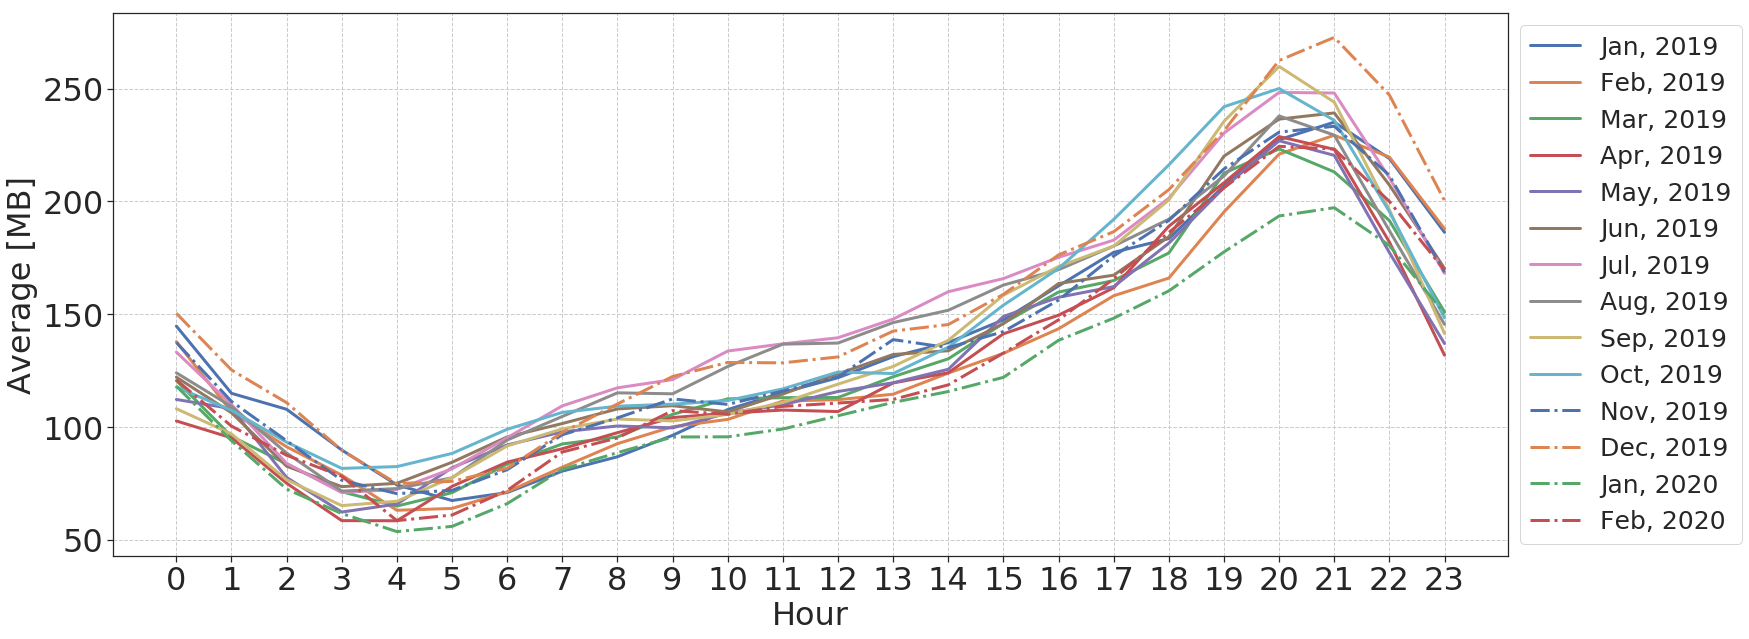
\includegraphics[width=0.48\linewidth]{figs/wenjun/download_wdays_before.png}%
    }
    \hspace{0.2cm}
    \subfloat[\textbf{Pre-lockdown weekends.} Average volume of downloaded data per test unit, broken down by the hour of the day, on weekends in the pre-lockdown time period. \label{download-b}]{%
        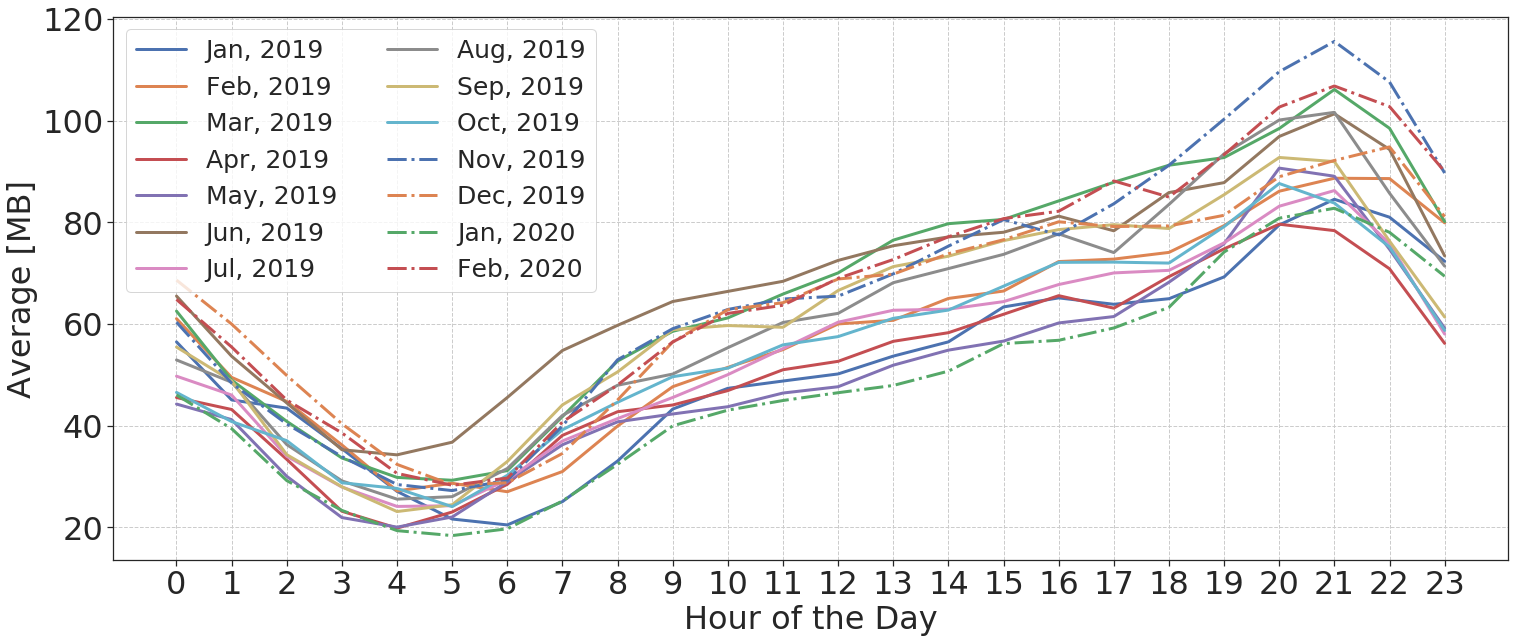
\includegraphics[width=0.48\linewidth]{figs/wenjun/download_wends_before.png}%
    }
    \\
    \subfloat[\textbf{Lockdown weekdays.} Average volume of downloaded data per test unit, broken down by the hour of the day, on weekdays in the lockdown time period. \label{download-c}]{%
        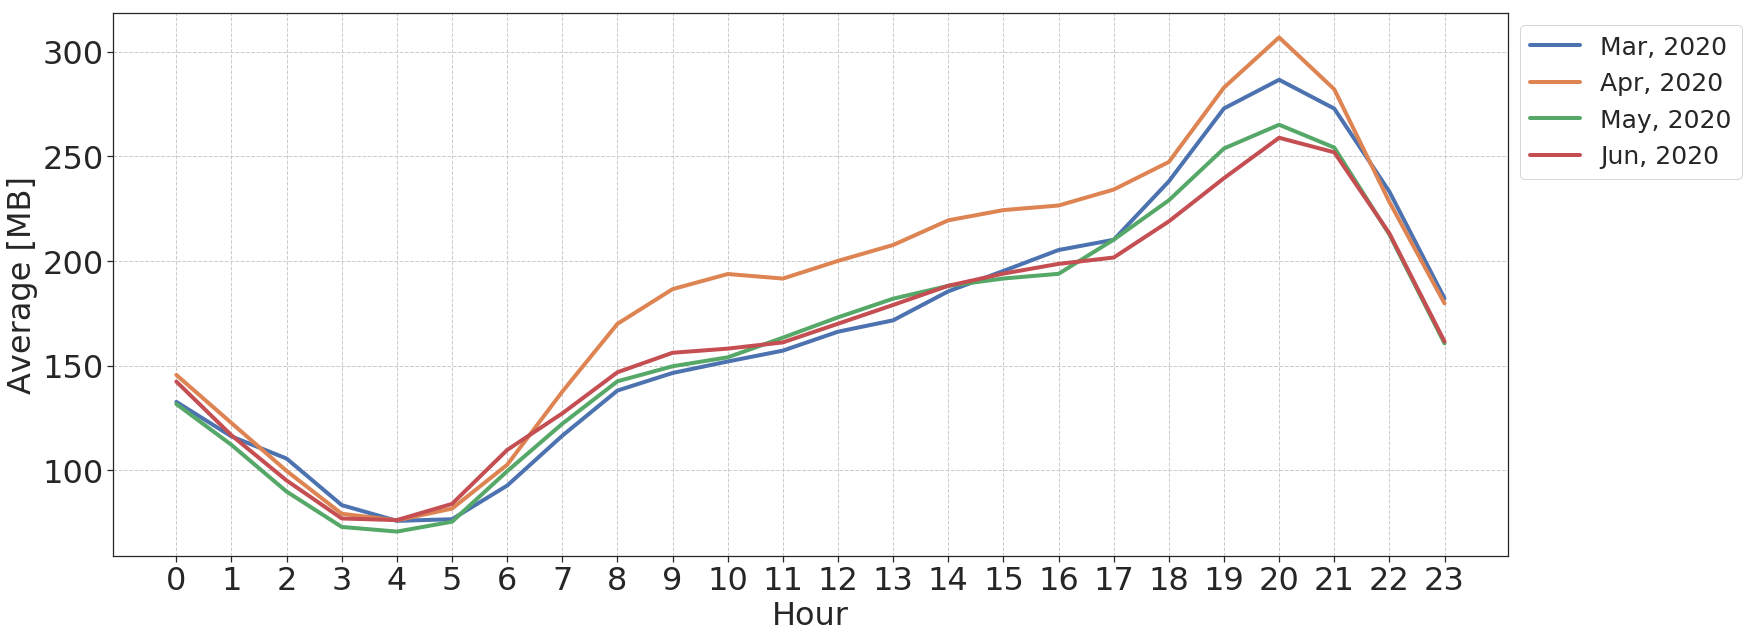
\includegraphics[width=0.48\linewidth]{figs/wenjun/download_wdays_after.png}%
    }
    \hspace{0.2cm}
    \subfloat[\textbf{Lockdown weekends.} Average volume of downloaded data per test unit, broken down by the hour of the day, on weekends in the lockdown time period. \label{download-d}]{%
        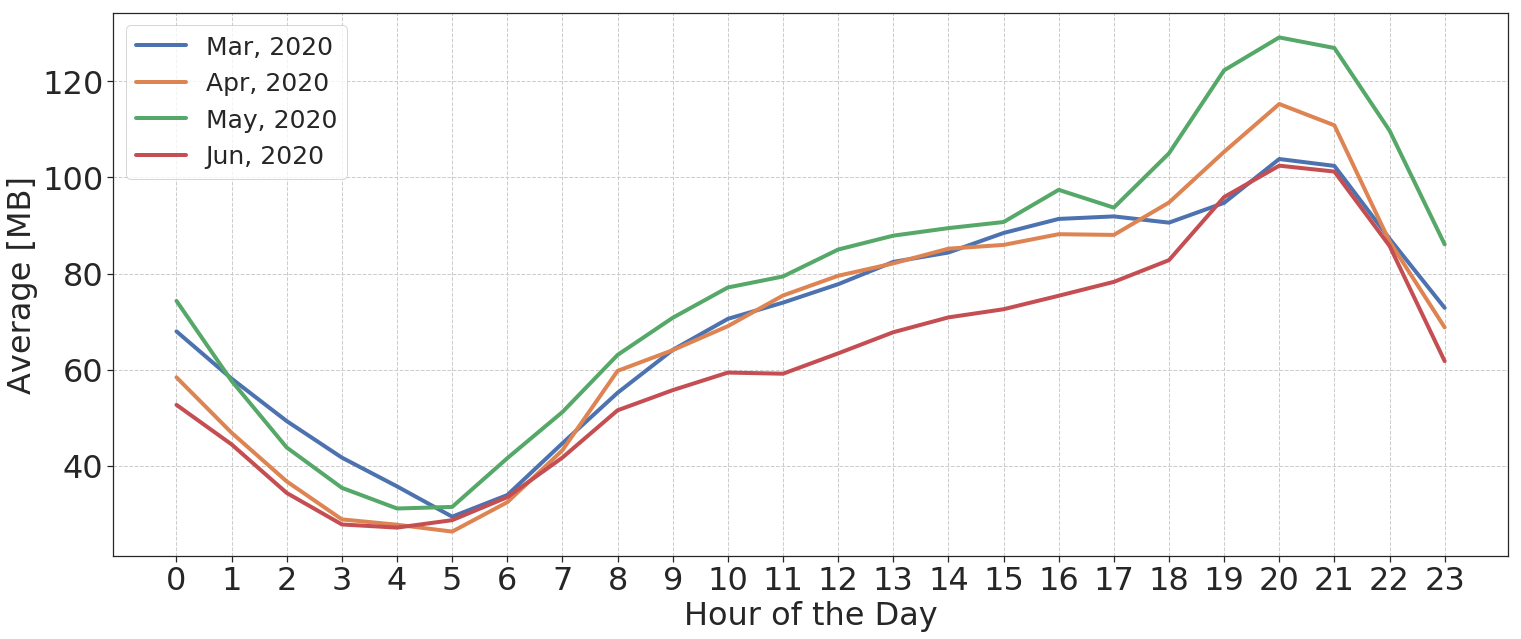
\includegraphics[width=0.48\linewidth]{figs/wenjun/download_wends_after.png}%
    }
    \\
    \subfloat[\textbf{2019 vs 2020 weekdays.} Average volume of downloaded data per test unit on weekdays in March-June compared between 2019 and 2020.
    \label{download-e}]{%
        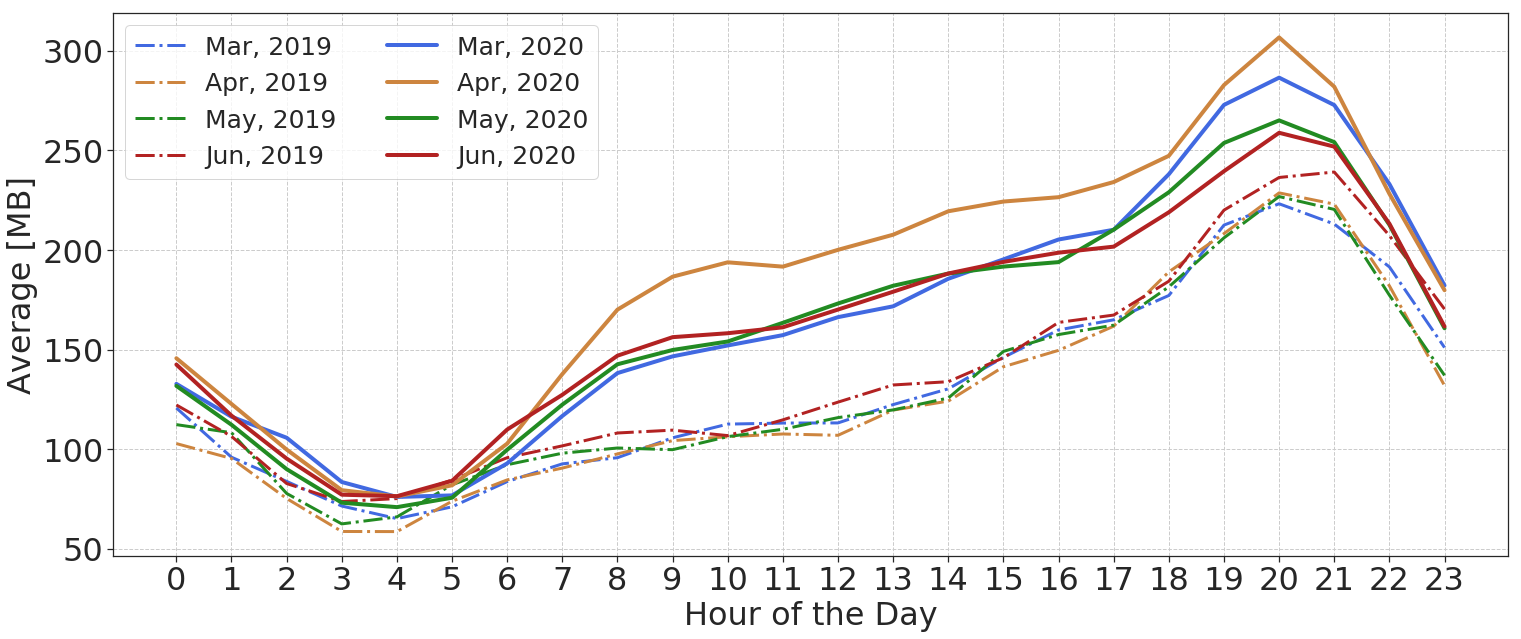
\includegraphics[width=0.48\linewidth]{figs/wenjun/download_wdays_compare_36.png}%
    }
    \hspace{0.2cm}
    \subfloat[\textbf{2019 vs 2020 weekends.} Average volume of downloaded data per test unit on weekends in March-June compared between 2019 and 2020.
    \label{download-f}]{%
        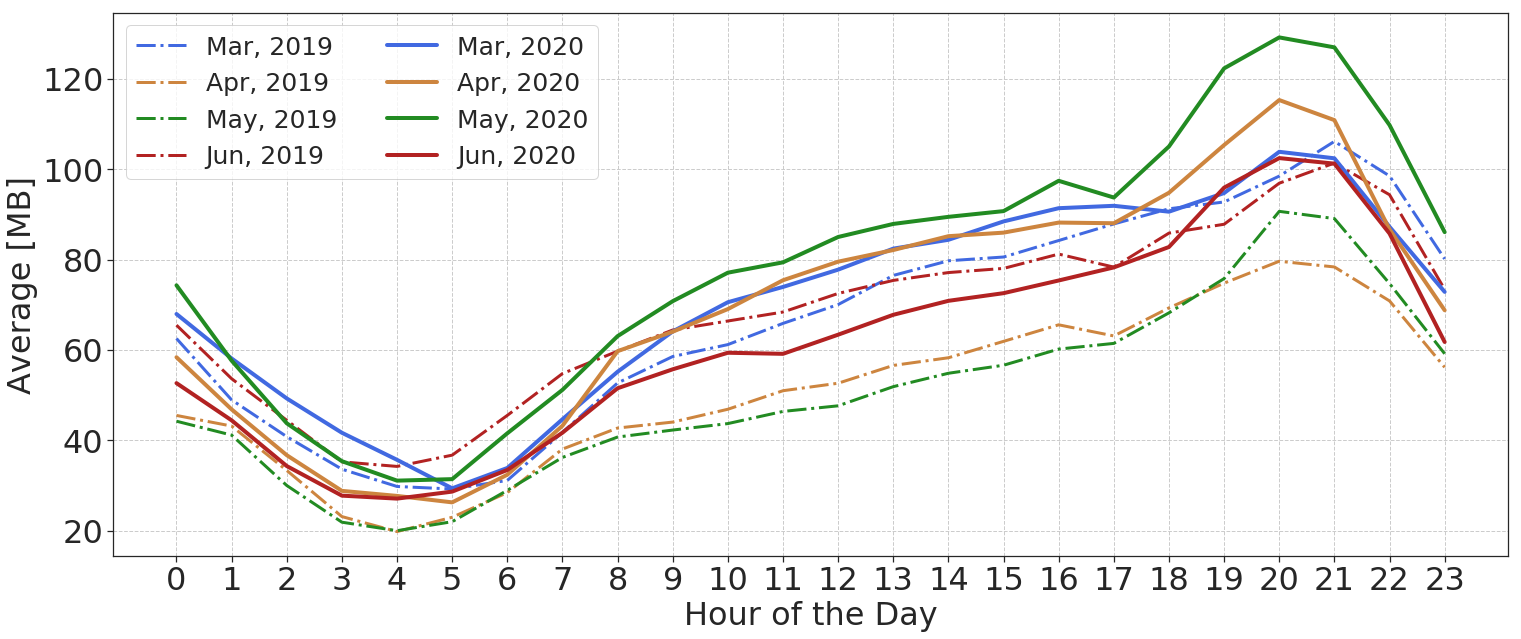
\includegraphics[width=0.48\linewidth]{figs/wenjun/download_wends_compare_36.png}%
    }
        
    \caption{Graphs comparing and contrasting the average hourly downloaded volume of data per test unit in various time periods. The peak is always between 18:00 and 22:00, which is the internet rush hour. The volumes in the lockdown time period are generally larger than the volumes in the pre-lockdown time period. Lockdown weekday traffic patterns start to resemble weekend patterns.
    }
    \label{fig:download-data-per-user-hours-fig}
\end{figure*}

\begin{figure*}[th]
    \centering
    \subfloat[\textbf{Pre-lockdown weekdays.} Average volume of uploaded data per test unit, broken down by the hour of the day, on weekdays in the pre-lockdown time period.
    \label{upload-a}]{%
        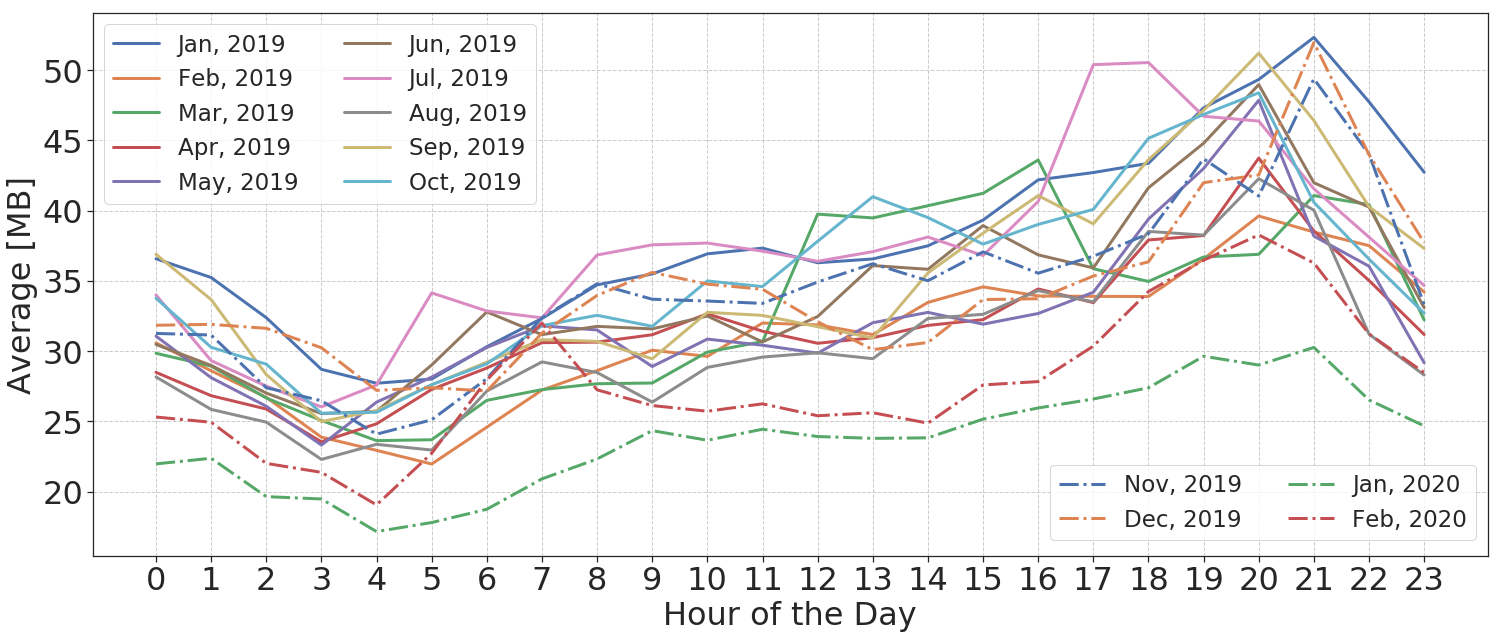
\includegraphics[width=0.48\linewidth]{figs/wenjun/upload_wdays_before.png}%
    }
    \hspace{0.2cm}
    \subfloat[\textbf{Pre-lockdown weekends.} Average volume of uploaded data per test unit, broken down by the hour of the day, on weekends in the pre-lockdown time period.
    \label{upload-b}]{%
        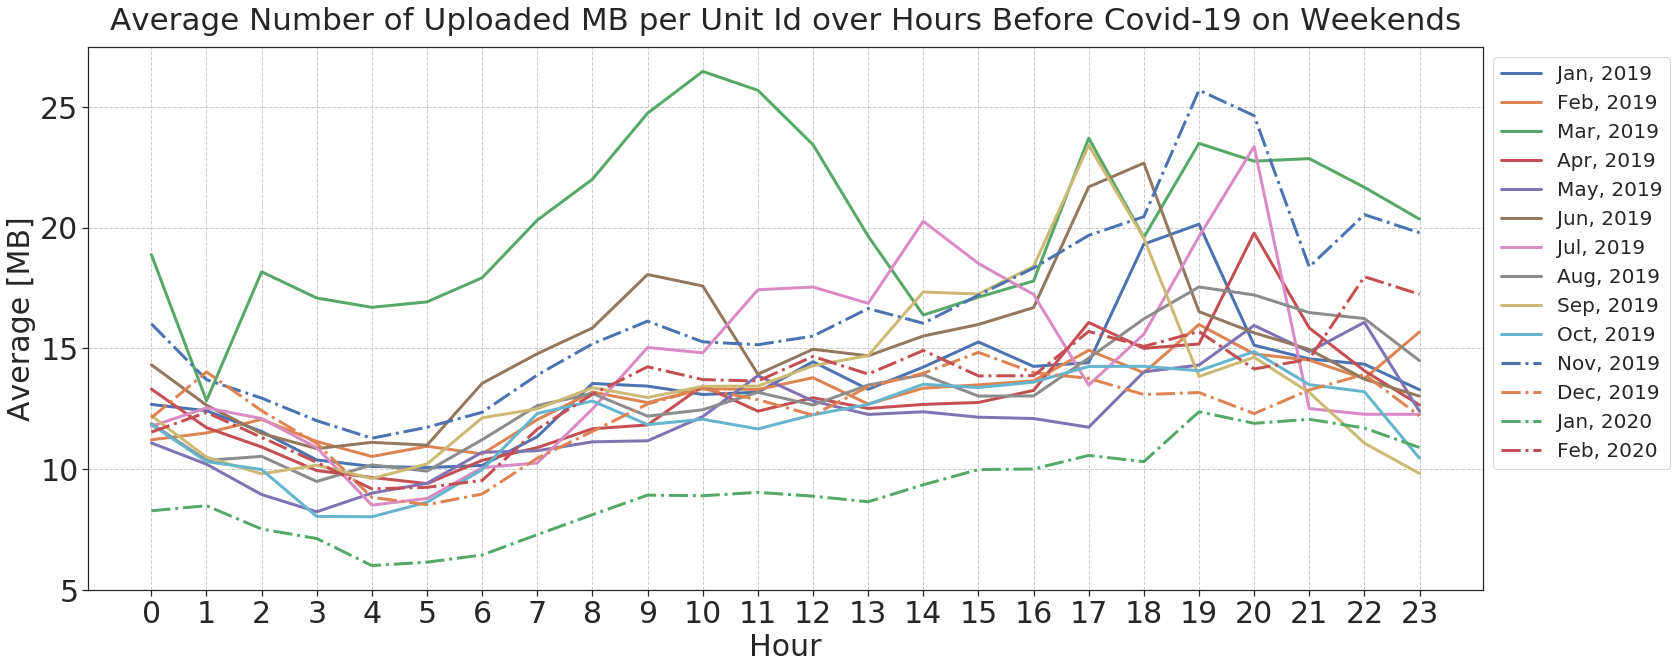
\includegraphics[width=0.48\linewidth]{figs/wenjun/upload_wends_before.png}%
    }
    \\
    \subfloat[\textbf{Lockdown weekdays.} Average volume of uploaded data per test unit, broken down by the hour of the day, on weekdays in the lockdown time period.
    \label{upload-c}]{%
        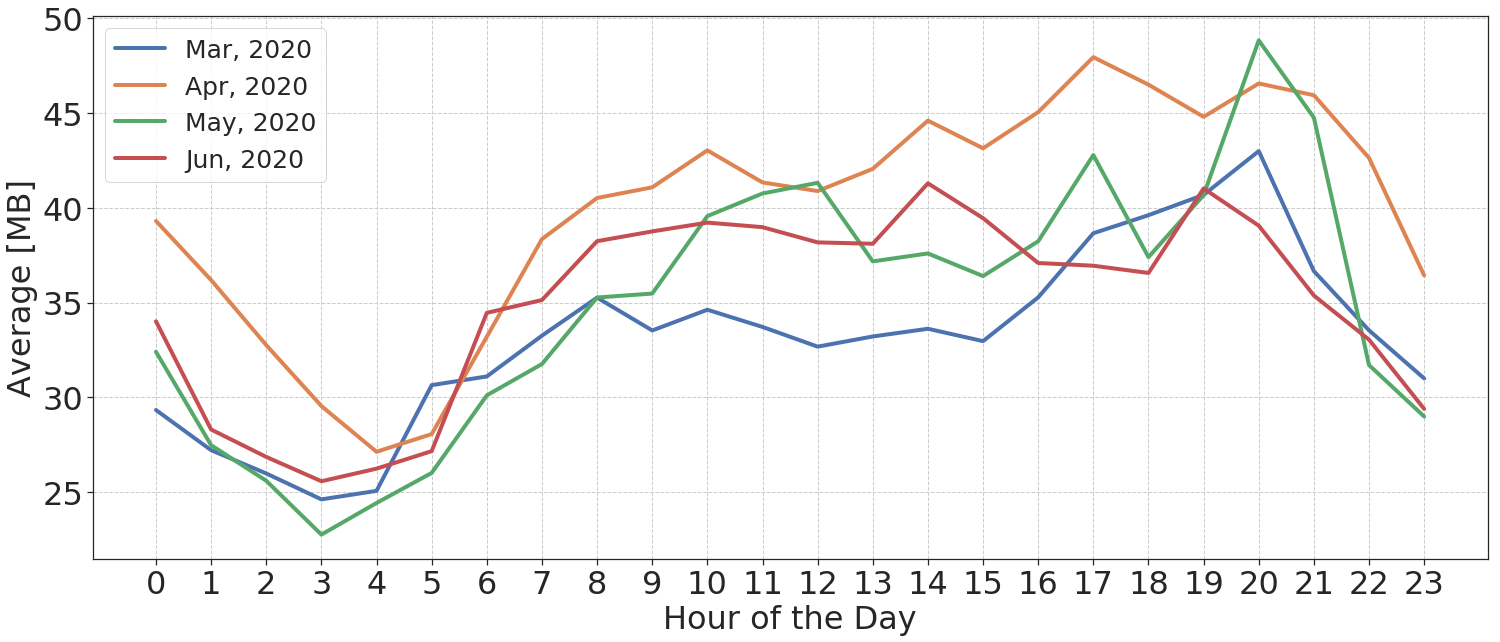
\includegraphics[width=0.48\linewidth]{figs/wenjun/upload_wdays_after.png}%
    }
    \hspace{0.2cm}
    \subfloat[\textbf{Lockdown weekends.} Average volume of uploaded data per test unit, broken down by the hour of the day, on weekends in the lockdown time period. \label{upload-d}]{%
        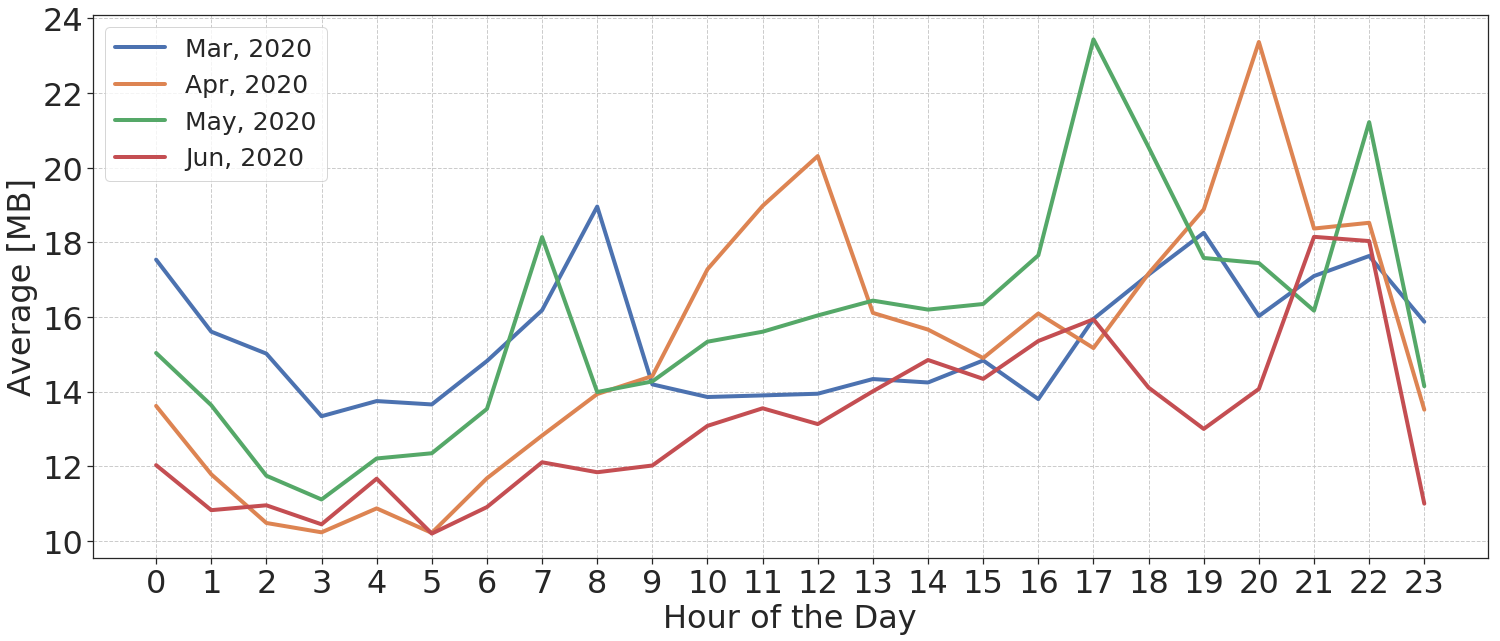
\includegraphics[width=0.48\linewidth]{figs/wenjun/upload_wends_after.png}%
    }
    \\
    \subfloat[\textbf{2019 vs 2020 weekdays.} Average volume of uploaded data per test unit on weekdays in March-June compared between 2019 and 2020.
    \label{upload-e}]{%
        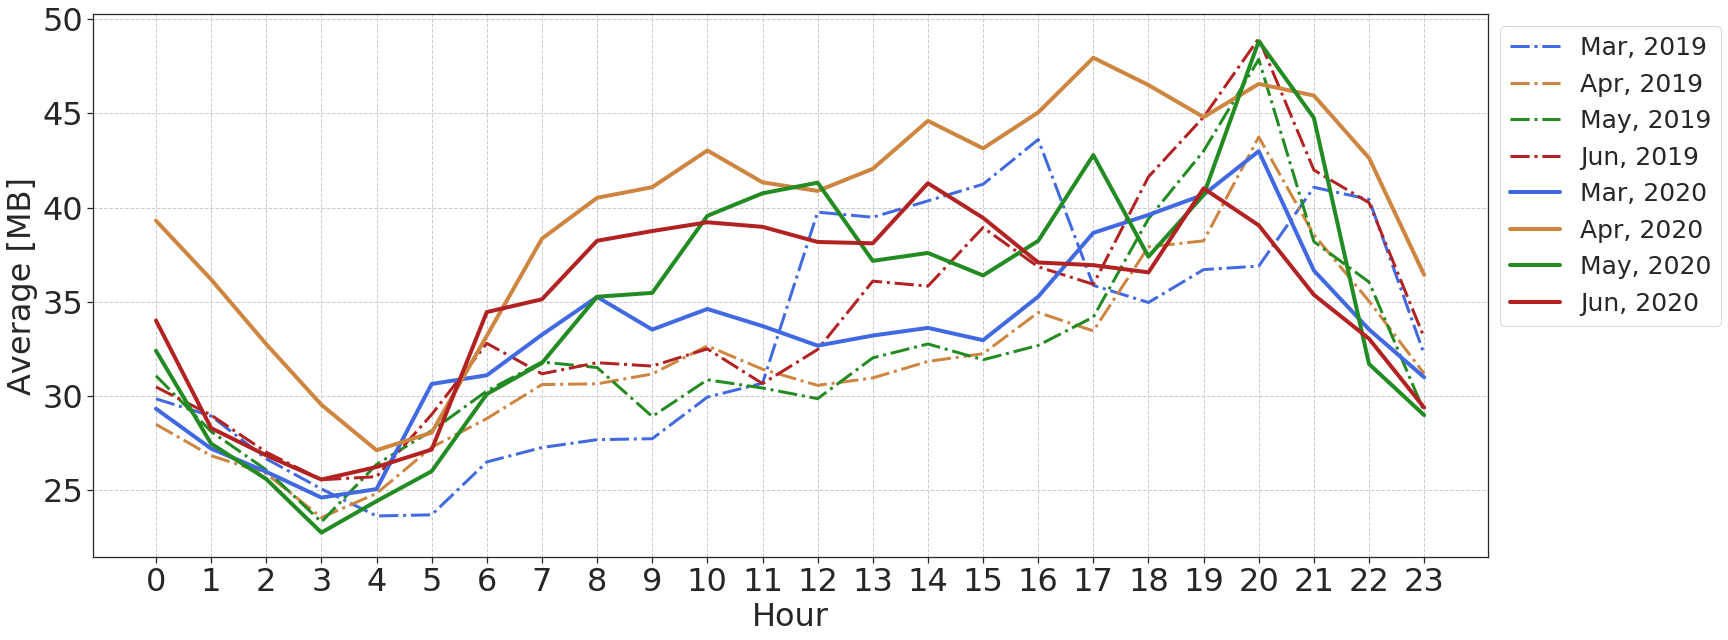
\includegraphics[width=0.48\linewidth]{figs/wenjun/upload_wdays_compare_36.png}%
    }
    \hspace{0.2cm}
    \subfloat[\textbf{2019 vs 2020 weekends.} Average volume of uploaded data per test unit on weekends in March-June compared between 2019 and 2020.
    \label{upload-f}]{%
        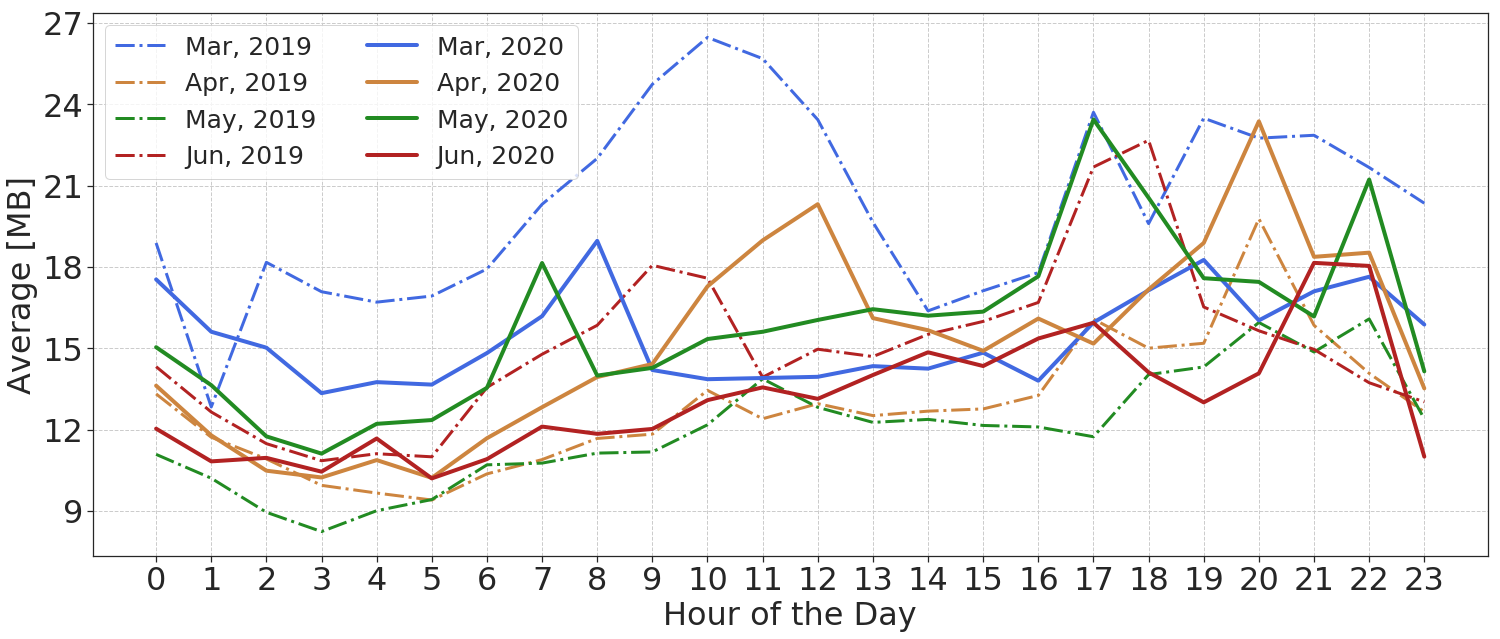
\includegraphics[width=0.48\linewidth]{figs/wenjun/upload_wends_compare_36.png}%
    }
        
    \caption{Graphs comparing and contrasting the average hourly upload volume of data per test unit in various time periods. Compared with download patterns, the lines in these graphs fluctuate more, especially on weekends. When comparing April and May between 2019 and 2020, we see an overall increase in uploaded data in 2020.}
  \label{fig:upload_data_per_user_hours_fig} 
\end{figure*}


\section{Hourly Data Usage Patterns}
\label{sec:hourly-data-usage-patterns}

Hourly data usage patterns (upload and download) could potentially provide insights into the behavior of fixed broadband internet users before and during the pandemic. Some applications such as music and video streaming generally increase the volume of downloaded data. Other applications such as VoIP, video conferencing, or networked games influence the volume of uploaded data.

In this section, we study the average hourly data usage per test unit from multiple perspectives and attempt to correlate with changing user behavior patterns during the lockdown. We contrast weekday and weekend patterns, analyze the differences in uploaded and downloaded traffic volumes, and compare with the data from the corresponding period of 2019 to eliminate potential seasonal differences.

% Say something about what data is being used in this section and how it is processed to generate the graphs.

\subsection{Download Analysis}
\label{sec:download-analysis}

As shown in Figure \ref{fig:download-data-per-user-hours-fig}, the patterns of average hourly downloaded volume of data per test unit are the same on weekdays and weekends whether before COVID-19 or after COVID-19. There is a peak between 18:00 and 22:00, which is the internet rush hour \cite{internetrushhour}. A likely explanation for this peak is post-workday internet consumption in the form of Youtube, Netflix, etc. 

According to the Figure \ref{download-e} and Figure \ref{download-f}, the average hourly downloaded volume of data per test unit after COVID-19 is larger than those before COVID-19. 

On weekdays (Figure \ref{download-e}), the gaps between average downloaded data per test unit from March to June in 2020 and average downloaded data per test unit in 2019 from 7:00 to 22:00 are more obvious than those from 22:00 to 7:00 next day. For the increase from 7:00 to 18:00, the possible reasons are work from home and online learning. Since the work-from-home period mainly took place from April and May \cite{remotework}, the average hourly downloaded volume of data per test unit in April increases the most in 2020. The increase from 18:00 to 22:00 is likely due to gathering and social contact restriction, and then people are not allowed to hang out with friends and dine in at the restaurant after work \cite{lockdownsguide}. Instead, people are supposed to stay at home. Watching streaming video or other recreational activities that require internet may be the first choice for most of the people, and these online activities will consume a lot of downloaded data. 22:00 to 7:00 the next day are generally reserved for sleep, so the lack of difference between downloaded data usage in these hours before and after COVID-19 is unsurprising. 

On weekends (Figure \ref{download-f}), there is a small rise for the average hourly downloaded volume of data per test unit in March, and the increases in April and May are substantial. In June, the average hourly downloaded data per test unit in 2020 is not always larger than those in 2019. This pattern coincides with the policies related to COVID-19 in the United States: the height of restriction was at the end of March and the beginning of April, and some restrictions such as stay-at-home order were ended in the mid-late of May or in June at most of the states \cite{covid19restriction}. We speculate that in April and May, people might need to stay at home and use internet the most. Since the restriction took place in the middle of March, the average hourly downloaded volume of data per test unit was not affected too much, and in June, some of the restrictions ended and people might be able to reschedule the outdoor activities. Therefore, we may be able to conclude that people use more internet and download more data because of COVID-19 and its related policies (e.g., lockdown, quarantine, work from home, etc.). 

\subsection{Upload Analysis}
\label{sec:upload-analysis}

As evidenced in Figure \ref{fig:upload_data_per_user_hours_fig}, compare with the patterns in average hourly downloaded data, the lines in the uploaded data graphs are more fluctuating, especially the patterns for the uploaded data on weekends.

Similar to the average hourly downloaded volume of data per test unit, we compare the average hourly uploaded data from March to June in 2020, the period after COVID-19, with those from March to June in 2019. The average hourly uploaded volume of data per test unit in April and May 2020 are larger than those in 2019, but in March and June, that is not the case (Figure \ref{upload-e} and \ref{upload-f}). The possible reasons might be similar to those of downloaded data: the peak of shelter-in-place and stay-at-home were 
at the end of March and the beginning of April, and the restrictions were ended in the mid-late of May or in June at some states \cite{covid19restriction}. On weekdays, potentially because of the policies such as work-from-home, the average upload data per test unit at daytime in April, May, and June 2020 are observed much larger than those in April, May, and June 2019. On weekends, the increase of uploaded data is relatively smaller than that on weekdays. One possible reason could be that weekend is a time to have a rest.  